\documentclass[a4paper,twocolumn,11pt,unpublished]{quantumarticle}
\pdfoutput=1
\usepackage[utf8]{inputenc}
\usepackage[english]{babel}
\usepackage[T1]{fontenc}
\usepackage{amsmath,amssymb,amsthm,mathtools}
\usepackage{booktabs}
\usepackage{graphicx}
\usepackage{microtype}
\usepackage{hyperref}
\usepackage[numbers,sort&compress]{natbib}
\usepackage{tikz}
\usepackage{xcolor}
\usetikzlibrary{arrows.meta,positioning,fit}

\newtheorem{proposition}{Proposition}
\newcommand{\bits}{\{0,1\}}
\newcommand{\E}{\mathbb{E}}
\newcommand{\mmd}{\operatorname{MMD}}
\newcommand{\TVD}{\operatorname{TVD}}
\newcommand{\supp}{\operatorname{supp}}
\definecolor{paperblue}{HTML}{0072B2}
\definecolor{paperorange}{HTML}{D55E00}
\definecolor{papergreen}{HTML}{009E73}
\definecolor{paperpurple}{HTML}{CC79A7}

\title{Conditional Generation with Classically Trainable IQP Circuits}
\author{Author names withheld pending team verification}
\affiliation{Affiliations withheld pending team verification}

\begin{document}
\maketitle

\begin{abstract}
Conditional generation asks one model to produce a family of probability laws
indexed by an external condition.  We formalize a restrictive quantum version
of this task: the condition changes only a product-state input to one compiled
instantaneous quantum polynomial-time (IQP) circuit, while the diagonal gate
sequence and all trained phases remain fixed.  We call the model classically
trainable in the operational sense that selected Pauli observables, a
Conditional maximum mean discrepancy objective, and its phase gradients admit
classical estimators; we do not claim an efficient classical evaluator or
sampler for the full output law.  We record finite response-support and
observable-filter propositions as specializations and syntheses of established
quantum-circuit Fourier and IQP theory.  On an archived 19-qubit Gaussian
Hamming-profile benchmark, paired ten-seed intervals support conditional
control and aggregate interpolation to four unseen interior conditions:
dense conditioning improves mean profile total variation distance over
endpoint-only training by $0.0893$ (95\% interval $[0.0762,0.1007]$) and over
adjacent-condition lookup by $0.0284$ ($[0.0268,0.0302]$).  Lookup nevertheless
wins at one condition, and no bitstring-level interpolation advantage is
detected.  A preregistered 16-qubit Ising extension stopped at its
representability screen (median exact bitstring TVD $0.512$, threshold
$0.25$), before tuning or primary comparisons.  The present evidence therefore
establishes the product-state conditioning mechanism on a task-appropriate
profile statistic, but not full-bitstring Ising conditional generation.
\end{abstract}

\section{Introduction}

Conditional generative models represent a family $q_\theta(x\mid c)$ rather
than a single probability law.  In a circuit Born machine, the condition can
be introduced by recompiling gates, by modulating trained phases, or by
changing the prepared input.  This paper studies the last and most restrictive
deployment setting: every condition uses one gate sequence and one trained
phase vector; only a product-state preparation changes.

This restriction separates two questions that are easily conflated.  First,
can a fixed quantum circuit respond usefully to a condition encoded in its
input?  Second, can the quantities used during optimization be estimated
classically?  The second question does not answer whether the final bitstring
law can be evaluated or sampled efficiently on a classical computer.
Probabilistic simulation of selected observables is weaker than strong
simulation of the full output distribution
\cite{nestSimulatingQuantumComputers2011,niCommutingQuantumCircuits2012}.
Conversely, sampling-hardness results for IQP circuits rely on separate
complexity assumptions and do not follow from the experiments here
\cite{bremnerClassicalSimulation2011,bremnerAverageCase2016}.

The key construction is illustrated in Fig.~\ref{fig:pipeline}.  A scalar or
vector condition is mapped to local $R_Y$ angles, followed by one fixed IQP
circuit.  The product input supplies a tractable reference distribution for
selected Pauli estimators and a Fourier implementation of Conditional MMD.
Established results on quantum data encodings imply that such responses have
finite Fourier support
\cite{gilVidalInputRedundancy2020,schuldEffectDataEncoding2021,
casasMultidimensionalFourier2023}; the known IQP active-generator expansion
further restricts selected observable responses
\cite{recio-armengolTrainClassicalDeploy2026}.  We use these facts as an
explanatory boundary, not as a theorem-novelty claim.

We make three scoped contributions.  First, we define product-state-conditioned
IQP generation and audit the invariant compiled circuit explicitly.  Second,
we state the exact operational scope of classical training signals, including
the Hamming-kernel mask law and gradient estimator.  Third, we recompute paired
uncertainty intervals for an archived Gaussian Hamming-profile study and
preregister a compact 16-qubit Ising protocol with exact full-law evaluation.
The Gaussian evidence is positive for profile control and aggregate
interpolation.  The Ising protocol stops before its primary study because a
Separate-model representability screen fails its frozen thresholds.

We use \emph{conditional generalization} once in a narrow operational sense:
interpolation to unseen conditions strictly inside the training interval.
Hereafter we use \emph{interpolation}.  Extrapolation and broader distribution
shift are outside scope.

\begin{figure*}[t]
\centering
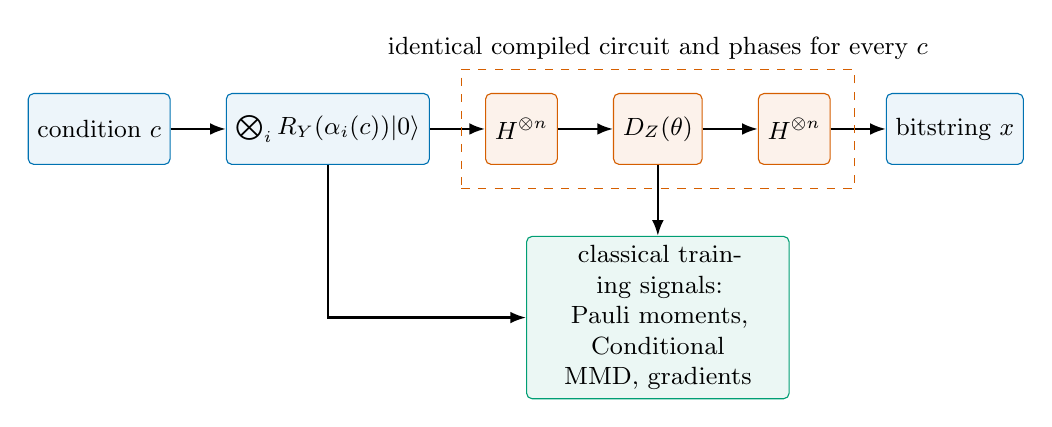
\begin{tikzpicture}[
  node distance=5mm and 7mm,
  box/.style={draw,rounded corners=2pt,minimum height=9mm,align=center,
    font=\small,fill=white},
  input/.style={box,draw=paperblue,fill=paperblue!7},
  fixed/.style={box,draw=paperorange,fill=paperorange!8},
  signal/.style={box,draw=papergreen,fill=papergreen!8,text width=3.1cm},
  arrow/.style={-{Latex[length=2mm]},thick}
]
\node[input] (c) {condition $c$};
\node[input,right=of c] (enc) {$\bigotimes_iR_Y(\alpha_i(c))|0\rangle$};
\node[fixed,right=of enc] (h1) {$H^{\otimes n}$};
\node[fixed,right=of h1] (d) {$D_Z(\theta)$};
\node[fixed,right=of d] (h2) {$H^{\otimes n}$};
\node[input,right=of h2] (sample) {bitstring $x$};
\draw[arrow] (c)--(enc);
\draw[arrow] (enc)--(h1);
\draw[arrow] (h1)--(d);
\draw[arrow] (d)--(h2);
\draw[arrow] (h2)--(sample);
\node[signal,below=9mm of d] (train) {classical training signals:\\Pauli moments, Conditional MMD, gradients};
\draw[arrow] (enc.south) |- (train.west);
\draw[arrow] (d.south) -- (train.north);
\node[draw=paperorange,dashed,fit=(h1)(d)(h2),inner sep=3mm,
  label=above:{\small identical compiled circuit and phases for every $c$}] {};
\end{tikzpicture}
\caption{Product-state-conditioned IQP generation.  The condition changes the
input angles but not the IQP generator bank, gate order, or trained phases.
Classical estimability of selected training signals is not a classical
full-output sampling claim.}
\label{fig:pipeline}
\end{figure*}

\section{Product-state-conditioned IQP generation}
\label{sec:model}

Let $g_j\in\bits^n$ identify a diagonal Pauli string
$Z_{g_j}=\bigotimes_i Z_i^{g_{j,i}}$.  For a fixed ordered generator bank
$G=(g_1,\ldots,g_m)$ and trained phases $\theta\in\mathbb R^m$, define
\begin{equation}
 D_Z(\theta)=\prod_{j=1}^{m}\exp(i\theta_j Z_{g_j}).
\end{equation}
The conditional Born law is
\begin{equation}
 \begin{split}
 q_\theta(x\mid c)=\bigg|\langle x|H^{\otimes n}D_Z(\theta)H^{\otimes n}\\
 {}\times\bigotimes_{i=1}^{n}R_Y(\alpha_i(c))|0\rangle\bigg|^2.
 \end{split}
 \label{eq:model}
\end{equation}
We use an affine encoding $\alpha(c)=b+Wc$.  The compiled sequence, $G$, and
$\theta$ are identical at every condition.  A deployment-signature test hashes
the coefficient vector, generator matrix, effective phases, and input angles
condition by condition; the fixed-input family must have invariant generators
and phases and non-invariant inputs.

We compare Eq.~\eqref{eq:model} with two parameter-matched shared models.  The
\emph{no-condition} control fixes the input at the anchor condition.  The
\emph{phase-conditioned} comparator also fixes the input but multiplies the
136 phases by a preregistered balanced feature bank containing 68 constant and
68 linear features.  It quantifies the cost of strict fixed deployment; the
fixed-input model is not required to beat it.  Separate models are used only as
a representability screen.

\section{Classical training signals}
\label{sec:training}

Our use of \emph{classically trainable} is deliberately operational.  It means
that selected Pauli-$Z$ expectations, the sampled Conditional MMD objective,
and phase gradients of that objective can be estimated with classical
probabilistic IQP methods for the declared finite budgets
\cite{nestSimulatingQuantumComputers2011,
recio-armengolIQPoptFastOptimization2025,
recio-armengolTrainClassicalDeploy2026}.  It does not mean that all output
probabilities are efficiently computable, that the final output is efficiently
sampleable classically, or that optimization has a favorable landscape.

For the Hamming radial basis kernel
$k_\sigma(x,y)=\exp[-d_H(x,y)/(2\sigma^2)]$, draw a mask
$a\in\bits^n$ with independent coordinates
\begin{equation}
 a_i\sim\operatorname{Bernoulli}(q_\sigma),\qquad
 q_\sigma=\frac{1-e^{-1/(2\sigma^2)}}{2}.
 \label{eq:mask-law}
\end{equation}
Then
\begin{equation}
 k_\sigma(x,y)=\E_a\left[(-1)^{a\cdot x}(-1)^{a\cdot y}\right].
 \label{eq:character-kernel}
\end{equation}
Equation~\eqref{eq:character-kernel} converts squared MMD into an average of
Pauli-character discrepancies.  Independent model/reference samples give the
usual unbiased U-statistic construction
\cite{grettonKernelTwoSample2012}; automatic differentiation of the finite
sample expression gives phase gradients.  Operator masks, model-reference
samples, target samples, minibatches, and validation streams use separately
derived seeds.

\section{Known response structure}
\label{sec:response}

The following propositions collect established structure in the notation of
Eq.~\eqref{eq:model}.  Complete derivations are supplied in the supplement.

\begin{proposition}[Affine product-input support]
For fixed $G,\theta,b,W$ and output $x$, the support of
$c\mapsto q_\theta(x\mid c)$ is contained in
\begin{equation}
 \Omega_{\mathrm{full}}(W)=
 \left\{\sum_{i=1}^{n}s_iw_i:s_i\in\{-1,0,1\}\right\},
 \label{eq:full-support}
\end{equation}
where $w_i^\mathsf{T}$ is row $i$ of $W$.
\end{proposition}

This is a direct specialization of multivariate circuit-Fourier theory
\cite{gilVidalInputRedundancy2020,schuldEffectDataEncoding2021,
casasMultidimensionalFourier2023}.  It is an inclusion: coincident frequencies
and coefficient cancellations can shrink the realized support.  It gives no
efficient procedure for evaluating the coefficients.

\begin{proposition}[Observable filter]
For the Pauli response $F_a(c)=\langle Z_a\rangle_c$, only generators with
$a\cdot g_j=1\pmod 2$ enter the known IQP active-generator expansion.  Grouping
their subsets by binary XOR mask $h$, a term survives on the real $R_Y$
product input only if $h\wedge a=0$.  Its condition frequencies are signed
sums of rows $w_i$ with $i\in\supp(a)\cup\supp(h)$.
\end{proposition}

This combines the active-generator formula of
Ref.~\cite{recio-armengolTrainClassicalDeploy2026} with the local identity
$\langle Y_i\rangle=0$.  It explains why a training observable can have a
smaller response spectrum than a full output probability.  For fixed $W$ both
spaces remain finite dimensional, so fixed width is not universally dense in
continuous conditional laws.

\section{Experiments}
\label{sec:experiments}

\subsection{Gaussian Hamming-profile benchmark}

The archived experiment uses 19 visible qubits and ten optimizer seeds.  Its
targets are condition-indexed Gaussian profiles over Hamming weight; states
within each weight shell are exchangeable.  The primary task metric is
therefore profile TVD.  Full bitstring TVD is also reported and is markedly
larger, exposing variation within shells that the task metric intentionally
quotients out.

The interpolation study trains a dense condition grid and evaluates four
unseen angles strictly between training angles.  Baselines are endpoint-only
training and an exact adjacent-condition lookup that chooses the better of the
two neighboring training-target laws.  We regenerated every legacy metric
exactly, then paired methods by optimizer seed and bootstrapped the ten paired
seed means 10,000 times.

Figure~\ref{fig:gaussian} summarizes the paired evidence.  At the two training
conditions, product-state conditioning improves mean profile TVD over the
no-condition control by $0.2751$ with 95\% interval
$[0.2667,0.2855]$.  On held-out conditions, dense conditioning improves mean
profile TVD over endpoint-only training by $0.0893$
($[0.0762,0.1007]$) and over adjacent lookup by $0.0284$
($[0.0268,0.0302]$).  These are aggregate claims: lookup has lower median
profile TVD at $0.15625\pi$.  For full bitstrings, the paired dense-minus-lookup
advantage is absent: baseline-minus-dense is $-0.0002$ with interval
$[-0.0026,0.0026]$.

\begin{figure*}[t]
\centering
\includegraphics[width=\textwidth]{foundations_figures/gaussian_evidence.pdf}
\caption{Gaussian Hamming-profile evidence.  (a) Paired seed-level improvement
over the no-condition control at training conditions.  (b) Aggregate held-out
profile-TVD improvement of dense conditioning over endpoint-only training and
adjacent lookup.  Error bars are 95\% paired bootstrap intervals over ten
optimizer seeds.}
\label{fig:gaussian}
\end{figure*}

\subsection{Preregistered 16-qubit Ising study}

The compact Ising benchmark uses exactly enumerated Gibbs laws of periodic
$4\times4$ random-coupling models.  Five training inverse temperatures are
$0.15$, $0.241\overline6$, $1/3$, $0.441\overline6$, and $0.55$; the four
held-out conditions are adjacent midpoints.  Development seeds are 606 and
707, primary seeds are 666, 101, 202, and 303, and seeds 404 and 505 are
unused reserves.  For each active instance and training condition, independent
categorical draws provide 5,000 training and 2,000 validation strings.  No
held-out training strings are generated.

All shared families use 16 visible qubits and the Complete 2-local bank of 136
trainable phases.  The estimator audit tests equal operator/reference budgets
$128,256,512,1024$.  The smallest budget, 128, passes all frozen criteria: at
$n=8$ its absolute loss bias is $0.0070$, mean gradient cosine $0.985$, and
normalized gradient RMSE $0.061$; at $n=16$ its repeated-loss coefficient of
variation is $0.079$ and median pairwise gradient cosine $0.950$.  A 100-update
preflight projects 14.95 seconds per 1,000-update run with 0.454 GB peak RSS on
the audit host, below the one-hour and 28-GiB limits.  These host measurements
are feasibility observations, not portable performance guarantees.

Before shared-family tuning, 12 Separate models test two development
instances, low/anchor/high conditions, and two optimizer seeds.  The frozen
gate requires median exact full-bitstring TVD at most 0.25 and every run at
most 0.35.  Figure~\ref{fig:ising-screen} shows that the median is 0.512 and
the maximum 0.866.  The gate therefore fails.  In accordance with the
manifest, no tuning run, primary run, held-out checkpoint evaluation, or Ising
publication test was executed.  This benchmark supplies a reproducible
negative boundary, not evidence that the proposed model works for the Ising
family.

\begin{figure*}[t]
\centering
\includegraphics[width=\textwidth]{foundations_figures/ising_representability.pdf}
\caption{Exact full-bitstring TVD for the 12-run Separate-model
representability screen.  Color identifies the two development instances and
marker shape the two optimizer seeds.  Both the median and every-cell
requirements are violated, so the preregistered study stops before tuning.}
\label{fig:ising-screen}
\end{figure*}

\begin{table*}[t]
\centering
\caption{Claim summary.  Positive statements are restricted to the archived
Gaussian Hamming-profile task.  All intervals are paired 95\% bootstrap
intervals over optimizer seeds.}
\label{tab:claims}
\begin{tabular}{p{3.5cm}p{4.2cm}p{2.4cm}p{4.7cm}}
\toprule
Claim & Statistic & Decision & Disclosure \\
\midrule
Gaussian profile conditional control & No-condition minus conditioned:
$0.2751$ $[0.2667,0.2855]$ & Supported & Two training conditions; ten seeds \\
Gaussian aggregate profile interpolation & Endpoint: $0.0893$
$[0.0762,0.1007]$; lookup: $0.0284$ $[0.0268,0.0302]$ & Supported & Lookup
wins at $0.15625\pi$ \\
Gaussian bitstring interpolation over lookup & $-0.0002$
$[-0.0026,0.0026]$ & Not supported & Profile result does not imply full-law advantage \\
Ising full-bitstring conditional generation & Screen median $0.512$; max
$0.866$ & Blocked & Frozen limits $0.25/0.35$; zero tuning and primary runs \\
Classical full-output sampling & Not tested or derived & Not claimed &
Classical training signals have narrower scope \\
\bottomrule
\end{tabular}
\end{table*}

\section{Limitations and reproducibility}

The strongest limitation is empirical: the compact Ising design fails before
the primary experiment, so this draft does not demonstrate full-bitstring
conditional generation on the intended physical benchmark.  The positive
Gaussian result concerns an exchangeable Hamming profile; bitstring TVD is
substantially less favorable and does not beat adjacent lookup in aggregate.
The experiments cover interpolation only.  The fixed finite response space
also rules out universal conditional expressivity at fixed width.

The complete protocol is frozen in
\texttt{configs/arxiv\_foundations\_v1.json}.  Its manifest digest, role-tagged
dataset hashes, estimator decision, runtime record, run reservations,
checkpoints, and exact-TVD rows are stored under
\texttt{results/arxiv-foundations-v1}.  The planner declares exactly 12
representability, 12 tuning, and 36 primary runs; failed predecessors make the
latter 48 identities ineligible.  Tests cover cardinalities, seed separation,
exact-draw determinism, role isolation, circuit signatures, estimator
boundaries, exact TVD, bootstrap pairing, gate boundaries, and a tiny complete
run.  Supplementary material gives commands, proofs, and full protocol tables.

\section{Conclusion}

Product-state conditioning provides a precise way to turn one compiled IQP
circuit into a conditional generator while retaining classical access to
selected observable-based training signals.  Established Fourier and IQP
structure explains both why condition responses are controlled and why this
access does not extend to full-output classical simulation.  On Gaussian
Hamming profiles, paired evidence supports conditional control and aggregate
within-range interpolation, with an explicit per-condition failure and no
bitstring-level advantage over lookup.  The preregistered Ising extension does
not pass its representability screen.  The immediate research direction is
therefore to diagnose full-law representability under a new, separately
versioned protocol before making any broader conditional-generation claim.

\section*{Data and code availability}

Source code, manifests, tests, and immutable numerical evidence are included
with this internal draft.  No external upload has been performed.

\section*{Release metadata}

Verified author names, affiliations, contribution statements, competing
interests, arXiv category and license, and final human proof approval have not
yet been supplied.  This document is not upload-ready.

\bibliographystyle{unsrtnat}
\bibliography{references}

\clearpage
\appendix
\section{Analytical details}
\label{app:analysis}

This appendix derives the response and estimator statements used in the main
text.  The derivations specialize established circuit-Fourier and
probabilistic-IQP results to the product-state-conditioned notation; they are
not presented as new central theorems.

\subsection{Full-probability response support}

One encoded qubit has density operator
\begin{equation}
 \begin{split}
 \rho_i(\alpha_i)={}&R_Y(\alpha_i)|0\rangle\!\langle0|R_Y(\alpha_i)^\dagger\\
 ={}&\tfrac12\left(I+\sin\alpha_i X+\cos\alpha_i Z\right).
 \end{split}
 \label{eq:local-density}
\end{equation}
Every entry of Eq.~\eqref{eq:local-density} is a linear combination of angle
frequencies $-1,0,+1$.  Tensoring and substituting
$\alpha_i(c)=b_i+w_i^\mathsf{T}c$ gives fixed matrices $A_s$ such that
\begin{equation}
 \rho(c)=\sum_{s\in\{-1,0,1\}^n}
 A_s e^{i\sum_i s_i b_i}
 e^{i(\sum_i s_iw_i)^\mathsf{T}c}.
\end{equation}
For a fixed unitary $U$ and outcome $x$,
$q(x\mid c)=\operatorname{Tr}[U^\dagger|x\rangle\!\langle x|U\rho(c)]$
is a fixed linear functional of $\rho(c)$ and introduces no new condition
frequency.  This proves the inclusion in Eq.~\eqref{eq:full-support}.  Zero
encoding rows, coincident sums, and coefficient cancellations can only shrink
the realized support.  The trace coefficient can still require exponential
work to evaluate.

\subsection{Pauli observable filter}

The final Hadamards map the measured $Z_a$ to $X_a$.  A diagonal generator
$Z_{g_j}$ with $a\cdot g_j=0\pmod2$ commutes with $X_a$ and cancels.  For an
active generator,
\begin{equation}
 e^{-i\theta_jZ_{g_j}}X_ae^{i\theta_jZ_{g_j}}
 =X_ae^{2i\theta_jZ_{g_j}}.
\end{equation}
Since the diagonal generators commute,
\begin{equation}
 \begin{split}
 D_Z(\theta)^\dagger X_aD_Z(\theta)={}&X_a
 \prod_{j:a\cdot g_j=1}\\
 &\left[\cos(2\theta_j)I+i\sin(2\theta_j)Z_{g_j}\right].
 \end{split}
 \label{eq:active-product-foundations}
\end{equation}
Expanding the product groups active subsets by the binary mask
$h=\bigoplus_{j\in S}g_j$.  Conjugating $X_aZ_h$ through the first Hadamards
produces local $Z_aX_h$ factors.  On the real product input,
\begin{equation}
 \langle X_i\rangle=\sin\alpha_i,\qquad
 \langle Z_i\rangle=\cos\alpha_i,\qquad
 \langle Y_i\rangle=0.
\end{equation}
Thus every term with $h\wedge a\ne0$ vanishes.  Surviving terms factor into
sines and cosines on $\supp(a)\cup\supp(h)$, and expanding them into
exponentials yields only signed sums of the corresponding encoding rows.

\subsection{Hamming-kernel mask identity}

For one bit, let $a\sim\operatorname{Bernoulli}(q)$.  Then
\begin{equation}
 \E_a[(-1)^{a(x-y)}]=
 \begin{cases}
 1,&x=y,\\
 1-2q,&x\ne y.
 \end{cases}
\end{equation}
Choosing $q=q_\sigma$ from Eq.~\eqref{eq:mask-law} makes
$1-2q=e^{-1/(2\sigma^2)}$.  Independence across bits therefore gives
Eq.~\eqref{eq:character-kernel}.  Let
$\phi_a(x)=(-1)^{a\cdot x}$.  For target samples $y_1,\ldots,y_T$ and model
samples $x_1,\ldots,x_R$, the fixed-mask unbiased squared discrepancy is
\begin{align}
 \widehat\Delta_a^2={}&
 \frac{1}{R(R-1)}\sum_{r\ne r'}\phi_a(x_r)\phi_a(x_{r'})
 \nonumber\\
 &+\frac{1}{T(T-1)}\sum_{t\ne t'}\phi_a(y_t)\phi_a(y_{t'})
 \nonumber\\
 &-\frac{2}{RT}\sum_{r,t}\phi_a(x_r)\phi_a(y_t).
 \label{eq:mask-u-stat}
\end{align}
Averaging Eq.~\eqref{eq:mask-u-stat} over masks, bandwidths, and conditions
gives the sampled Conditional MMD objective.  Differentiation acts only on the
model expectation because the target and mask laws do not depend on the phase
parameters.  This establishes estimator accessibility, not a lower bound on
gradient magnitude or an optimizer-convergence guarantee.

\section{Gaussian reanalysis}
\label{app:gaussian}

All archived Gaussian metrics were regenerated from the ten JSON/NPZ run
pairs.  The regenerated per-angle medians and aggregate medians agree exactly
with the existing machine-readable audit.  For each comparison we then
averaged the four held-out conditions within each optimizer seed, preserved
the method pairing, and resampled ten seed identities with replacement 10,000
times using seed 20260811.

\begin{table*}[t]
\centering
\caption{Paired Gaussian improvements.  Positive values favor product-state
conditioning or dense-grid training.}
\label{tab:gaussian-paired}
\begin{tabular}{llll}
\toprule
Metric & Comparison & Paired mean & 95\% interval \\
\midrule
Training profile TVD & no-condition $-$ conditioned & 0.27510 & [0.26667, 0.28548] \\
Training bitstring TVD & no-condition $-$ conditioned & 0.16500 & [0.15561, 0.17328] \\
Held-out profile TVD & endpoint-only $-$ dense & 0.08935 & [0.07617, 0.10069] \\
Held-out profile TVD & adjacent lookup $-$ dense & 0.02843 & [0.02678, 0.03021] \\
Held-out bitstring TVD & endpoint-only $-$ dense & 0.01923 & [0.00670, 0.03338] \\
Held-out bitstring TVD & adjacent lookup $-$ dense & $-0.00022$ & [$-0.00261$, 0.00255] \\
\bottomrule
\end{tabular}
\end{table*}

The aggregate profile interval against lookup is positive even though lookup
has lower median profile TVD at the held-out angle $0.15625\pi$.  This is why
the main text states an aggregate result and discloses the condition-level
failure.  The bitstring interval against lookup contains zero and cannot
support a bitstring interpolation claim.

\section{Frozen compact Ising protocol}
\label{app:ising-protocol}

The versioned manifest has digest
\begin{center}
\small\ttfamily
076f694fa1b84221e6bd733e4746d4f3\\
5fea0afd81fa75a1c8e155b45cb4347b
\end{center}
Its run allocation is non-transferable: 12 representability, 12 tuning, and 36
primary runs.  A separate 100-update runtime identity is not charged to those
60 study runs.

\begin{table*}[t]
\centering
\caption{Compact Ising run matrix and observed release state.}
\label{tab:ising-plan}
\begin{tabular}{p{3.2cm}p{2.5cm}p{4.4cm}p{1.8cm}p{2.3cm}}
\toprule
Stage & Instances & Optimizer seeds / candidates & Declared runs & State \\
\midrule
Runtime preflight & 606 & fixed-input, seed 0 & 1 & passed \\
Representability & 606, 707 & low/anchor/high $\times$ seeds 0,1 & 12 & failed \\
Tuning & 606, 707 & 3 families $\times$ 2 LR schedules & 12 & blocked, zero run \\
Primary & 666, 101, 202, 303 & 3 seeds $\times$ 3 families & 36 & blocked, zero run \\
\bottomrule
\end{tabular}
\end{table*}

The two tuning schedules are $0.003\rightarrow0.0003$ and
$0.01\rightarrow0.001$.  Every non-preflight run uses 1,000 Adam updates with
cosine decay, 256 samples per condition per minibatch, validation every 50
updates, and the lowest validation Conditional MMD checkpoint.  The phase
comparator uses the balanced constant/slope bank.  If tuning were eligible,
each family would select its schedule by median validation Conditional MMD,
with candidate identifier as the deterministic tie-breaker.

Exact Gibbs laws are enumerated over all 65,536 bitstrings.  Categorical draws
use separate derived seeds for training and validation.  Archives contain
5,000 training and 2,000 validation strings for each active instance and
training condition.  Held-out sample generation is forbidden; exact held-out
laws are exposed only to the evaluation-facing interface after checkpoint
selection.  Development, primary, and reserve instance sets are disjoint.

The estimator selector evaluates equal operator/reference budgets
$128,256,512,1024$.  A candidate passes only if all five frozen metrics pass;
the selector stops if no candidate passes and always chooses the smallest
passing budget.  At eight repetitions, all four passed and budget 128 was
selected.  The screen result in Fig.~\ref{fig:ising-screen} uses exact TVD after
each validation-selected checkpoint.  Its median 0.51222 and maximum 0.86644
violate both preregistered limits, creating an immutable failed decision that
makes the tuning and primary planners ineligible.

Had the primary study been released, every frozen model would have been
evaluated at all five training and four held-out inverse temperatures.  The
binding conditional-control rule required fixed-input median training TVD at
most 0.35, a positive 95\% lower bound for no-condition minus fixed-input TVD,
and wins in at least 75\% of the 20 instance--training-condition cells after
optimizer-seed averaging.  The interpolation rule required positive lower
bounds against both no-condition and exact adjacent-target lookup, wins in at
least 75\% of the 16 instance--held-out cells, and lookup improvement in at
least three of four instance means.  These rules were implemented and tested
but not evaluated on absent primary results.

\section{Reproduction and integrity checks}
\label{app:reproduction}

From the repository root, first run \texttt{uv run pytest -q} and
\texttt{uv run ruff check src scripts tests}.  Regenerate the Gaussian and
figure evidence with \texttt{uv run python} followed by
\path{scripts/reanalyze_foundations_gaussian.py} and
\path{scripts/plot_foundations_evidence.py}, respectively.

The data, estimator audit, and stopped stages were produced with
\texttt{uv run python} and, in order,
\path{scripts/prepare_foundations_campaign.py},
\path{scripts/run_foundations_estimator.py}, and
\path{scripts/run_foundations_study.py} with arguments \texttt{runtime} and
\texttt{representability}.
Rerunning a completed immutable command refuses to rewrite its artifact.  The
campaign store rejects undeclared identities, foreign manifest digests,
duplicate reservations, missing checkpoint state, and partial result reuse.
The failed representability record blocks both
\texttt{run\_foundations\_study.py tuning} and
\texttt{run\_foundations\_study.py primary} before a new reservation is made.

To compile the manuscript in a clean temporary directory, copy
\texttt{paper/main.tex}, \texttt{paper/supplement.tex},
\texttt{paper/references.bib}, the \texttt{quantumarticle} class files, and the
two PDFs in \texttt{paper/foundations\_figures}; then run
\texttt{latexmk -pdf main.tex}.  The automated build additionally uses
nonstop and halt-on-error flags.
The arXiv source archive additionally includes a checksum manifest and excludes
auxiliary build products.


\end{document}
